\documentclass[sts]{imsart}

\RequirePackage[OT1]{fontenc}
\usepackage{amsthm,amsmath,amssymb,natbib,xspace,graphicx}
\RequirePackage[colorlinks,citecolor=blue,urlcolor=blue]{hyperref}

% settings
%\pubyear{2005}
%\volume{0}
%\issue{0}
%\firstpage{1}
%\lastpage{8}

\startlocaldefs
\numberwithin{equation}{section}
\theoremstyle{plain}
\newtheorem{thm}{Theorem}[section]

%%FJH defs
\DeclareSymbolFont{GreekLetters}{OML}{cmr}{m}{it} %Provide missing letters
\DeclareSymbolFont{UpSfGreekLetters}{U}{cmss}{m}{n} %Provide missing letters
\DeclareMathSymbol{\varrho}{\mathalpha}{GreekLetters}{"25}
\DeclareMathSymbol{\UpSfLambda}{\mathalpha}{UpSfGreekLetters}{"03}
\DeclareMathSymbol{\UpSfSigma}{\mathalpha}{UpSfGreekLetters}{"06}
%\newcommand{\bvec}[1]{\boldsymbol{#1}}
\providecommand{\mathbold}{\boldsymbol}
\newcommand{\bvec}[1]{\mathbold{#1}}
%\newcommand{\bvec}[1]{\text{\boldmath$#1$}}
\newcommand{\avec}[1]{\vec{#1}}
%\renewcommand{\vec}[1] {\text{\boldmath$#1$}}
%\renewcommand{\vec}[1]{\ensuremath{\mathbf{#1}}}
%\newcommand{\vecsym}[1]{\ensuremath{\boldsymbol{#1}}}
\newcommand{\vecsym}[1]{\ensuremath{\mathbold{#1}}}
\def\bbl{\text{\boldmath$\{$}}
\def\bbr{\text{\boldmath$\}$}}
\newcommand{\bbrace}[1]{\bbl #1 \bbr}
\newcommand{\bbbrace}[1]{\mathopen{\pmb{\bigg\{}}#1\mathclose{\pmb{\bigg\}}}}
%\def\bbl{\boldsymbol{\left \{}}
%\def\bbr{\boldsymbol{\right \}}}
\def\betahat{\hat\beta}
%\def\e{\text{e}}
%\def\E{\text{E}}
\newcommand{\dif}{{\rm d}}

\newlength{\overwdth}
\def\overstrike#1{ 
\settowidth{\overwdth}{#1}\makebox[0pt][l]{\rule[0.5ex]{\overwdth}{0.1ex}}#1}

\def\abs#1{\ensuremath{\left \lvert #1 \right \rvert}}
\newcommand{\normabs}[1]{\ensuremath{\lvert #1 \rvert}}
\newcommand{\bigabs}[1]{\ensuremath{\bigl \lvert #1 \bigr \rvert}}
\newcommand{\Bigabs}[1]{\ensuremath{\Bigl \lvert #1 \Bigr \rvert}}
\newcommand{\biggabs}[1]{\ensuremath{\biggl \lvert #1 \biggr \rvert}}
\newcommand{\Biggabs}[1]{\ensuremath{\Biggl \lvert #1 \Biggr \rvert}}
\newcommand{\norm}[2][{}]{\ensuremath{\left \lVert #2 \right \rVert}_{#1}}
\newcommand{\normnorm}[2][{}]{\ensuremath{\lVert #2 \rVert}_{#1}}
\newcommand{\bignorm}[2][{}]{\ensuremath{\bigl \lVert #2 \bigr \rVert}_{#1}}
\newcommand{\Bignorm}[2][{}]{\ensuremath{\Bigl \lVert #2 \Bigr \rVert}_{#1}}
\newcommand{\biggnorm}[2][{}]{\ensuremath{\biggl \lVert #2 \biggr \rVert}_{#1}}
\newcommand{\ip}[3][{}]{\ensuremath{\left \langle #2, #3 \right \rangle_{#1}}}

\newcommand{\bigvecpar}[3]{\ensuremath{\bigl ( #1 \bigr )_{#2}^{#3}}}
\newcommand{\Bigvecpar}[3]{\ensuremath{\Bigl ( #1 \Bigr )_{#2}^{#3}}}
\newcommand{\biggvecpar}[3]{\ensuremath{\biggl ( #1 \biggr )_{#2}^{#3}}}
\newcommand{\bigpar}[1]{\ensuremath{\bigl ( #1 \bigr )}}
\newcommand{\Bigpar}[1]{\ensuremath{\Bigl ( #1 \Bigr )}}
\newcommand{\biggpar}[1]{\ensuremath{\biggl ( #1 \biggr )}}

\newcommand{\IIDsim}{\overset{\textup{IID}}{\sim}}

\DeclareMathOperator{\success}{succ}
\DeclareMathOperator{\sinc}{sinc}
\DeclareMathOperator{\sech}{sech}
\DeclareMathOperator{\csch}{csch}
\DeclareMathOperator{\dist}{dist}
\DeclareMathOperator{\spn}{span}
\DeclareMathOperator{\sgn}{sgn}
\DeclareMathOperator*{\rmse}{rmse}
\DeclareMathOperator{\Prob}{\mathbb{P}}
\DeclareMathOperator{\Ex}{\mathbb{E}}
\DeclareMathOperator{\rank}{rank}
\DeclareMathOperator{\erfc}{erfc}
\DeclareMathOperator{\erf}{erf}
\DeclareMathOperator{\cov}{cov}
\DeclareMathOperator{\cost}{cost}
\DeclareMathOperator{\comp}{comp}
\DeclareMathOperator{\corr}{corr}
\DeclareMathOperator{\diag}{diag}
\DeclareMathOperator{\var}{var}
\DeclareMathOperator{\opt}{opt}
\DeclareMathOperator{\brandnew}{new}
\DeclareMathOperator{\std}{std}
\DeclareMathOperator{\kurt}{kurt}
\DeclareMathOperator{\med}{med}
\DeclareMathOperator{\vol}{vol}
\DeclareMathOperator{\bias}{bias}
\DeclareMathOperator*{\argmax}{argmax}
\DeclareMathOperator*{\argmin}{argmin}
\DeclareMathOperator{\sign}{sign}
\DeclareMathOperator{\spann}{span}
\DeclareMathOperator{\cond}{cond}
\DeclareMathOperator{\trace}{trace}
\DeclareMathOperator{\Si}{Si}
%\DeclareMathOperator{\diag}{diag}
\DeclareMathOperator{\col}{col}
\DeclareMathOperator{\nullspace}{null}
\DeclareMathOperator{\Order}{{\mathcal O}}
%\DeclareMathOperator{\rank}{rank}

\newcommand{\vzero}{\bvec{0}}
\newcommand{\vone}{\bvec{1}}
\newcommand{\vinf}{\bvec{\infty}}
\newcommand{\va}{\bvec{a}}
\newcommand{\vA}{\bvec{A}}
\newcommand{\vb}{\bvec{b}}
\newcommand{\vB}{\bvec{B}}
\newcommand{\vc}{\bvec{c}}
\newcommand{\vd}{\bvec{d}}
\newcommand{\vD}{\bvec{D}}
\newcommand{\ve}{\bvec{e}}
\newcommand{\vf}{\bvec{f}}
\newcommand{\vF}{\bvec{F}}
\newcommand{\vg}{\bvec{g}}
\newcommand{\vG}{\bvec{G}}
\newcommand{\vh}{\bvec{h}}
\newcommand{\vi}{\bvec{i}}
\newcommand{\vj}{\bvec{j}}
\newcommand{\vk}{\bvec{k}}
\newcommand{\vK}{\bvec{K}}
\newcommand{\vl}{\bvec{l}}
\newcommand{\vell}{\bvec{\ell}}
\newcommand{\vL}{\bvec{L}}
\newcommand{\vm}{\bvec{m}}
\newcommand{\vp}{\bvec{p}}
\newcommand{\vq}{\bvec{q}}
\newcommand{\vr}{\bvec{r}}
\newcommand{\vs}{\bvec{s}}
\newcommand{\vS}{\bvec{S}}
\newcommand{\vt}{\bvec{t}}
\newcommand{\vT}{\bvec{T}}
\newcommand{\vu}{\bvec{u}}
\newcommand{\vU}{\bvec{U}}
\newcommand{\vv}{\bvec{v}}
\newcommand{\vV}{\bvec{V}}
\newcommand{\vw}{\bvec{w}}
\newcommand{\vW}{\bvec{W}}
\newcommand{\vx}{\bvec{x}}
\newcommand{\vX}{\bvec{X}}
\newcommand{\vy}{\bvec{y}}
\newcommand{\vY}{\bvec{Y}}
\newcommand{\vz}{\bvec{z}}
\newcommand{\vZ}{\bvec{Z}}

\newcommand{\ai}{\avec{\imath}}
\newcommand{\ak}{\avec{k}}
\newcommand{\avi}{\avec{\bvec{\imath}}}
\newcommand{\at}{\avec{t}}
\newcommand{\avt}{\avec{\vt}}
\newcommand{\ax}{\avec{x}}
\newcommand{\ah}{\avec{h}}
\newcommand{\akappa}{\avec{\kappa}}
\newcommand{\avx}{\avec{\vx}}
\newcommand{\ay}{\avec{y}}
\newcommand{\avy}{\avec{\vy}}
\newcommand{\avz}{\avec{\vz}}
\newcommand{\avzero}{\avec{\vzero}}
\newcommand{\aomega}{\avec{\omega}}
\newcommand{\avomega}{\avec{\vomega}}
\newcommand{\anu}{\avec{\nu}}
\newcommand{\avnu}{\avec{\vnu}}
\newcommand{\aDelta}{\avec{\Delta}}
\newcommand{\avDelta}{\avec{\vDelta}}

\newcommand{\valpha}{\bvec{\alpha}}
\newcommand{\vbeta}{\bvec{\beta}}
\newcommand{\vgamma}{\bvec{\gamma}}
\newcommand{\vGamma}{\bvec{\Gamma}}
\newcommand{\vdelta}{\bvec{\delta}}
\newcommand{\vDelta}{\bvec{\Delta}}
\newcommand{\vphi}{\bvec{\phi}}
\newcommand{\vvphi}{\bvec{\varphi}}
\newcommand{\vomega}{\bvec{\omega}}
\newcommand{\vlambda}{\bvec{\lambda}}
\newcommand{\vmu}{\bvec{\mu}}
\newcommand{\vnu}{\bvec{\nu}}
\newcommand{\vpsi}{\bvec{\psi}}
\newcommand{\vepsilon}{\bvec{\epsilon}}
\newcommand{\veps}{\bvec{\varepsilon}}
\newcommand{\veta}{\bvec{\eta}}
\newcommand{\vxi}{\bvec{\xi}}
\newcommand{\vtheta}{\bvec{\theta}}
\newcommand{\vtau}{\bvec{\tau}}
\newcommand{\vzeta}{\bvec{\zeta}}

\newcommand{\hA}{\widehat{A}}
\newcommand{\hvb}{\hat{\vb}}
\newcommand{\hcc}{\widehat{\cc}}
\newcommand{\hD}{\widehat{D}}
\newcommand{\hE}{\widehat{E}}
\newcommand{\hf}{\widehat{f}}
\newcommand{\hF}{\widehat{F}}
\newcommand{\hg}{\hat{g}}
\newcommand{\hvf}{\widehat{\bvec{f}}}
\newcommand{\hh}{\hat{h}}
\newcommand{\hH}{\widehat{H}}
\newcommand{\hi}{\hat{\imath}}
\newcommand{\hI}{\hat{I}}
\newcommand{\hci}{\widehat{\ci}}
\newcommand{\hj}{\hat{\jmath}}
\newcommand{\hp}{\hat{p}}
\newcommand{\hP}{\widehat{P}}
\newcommand{\hS}{\widehat{S}}
\newcommand{\hv}{\hat{v}}
\newcommand{\hV}{\widehat{V}}
\newcommand{\hx}{\hat{x}}
\newcommand{\hX}{\widehat{X}}
\newcommand{\hvX}{\widehat{\vX}}
\newcommand{\hy}{\hat{y}}
\newcommand{\hvy}{\hat{\vy}}
\newcommand{\hY}{\widehat{Y}}
\newcommand{\hvY}{\widehat{\vY}}
\newcommand{\hZ}{\widehat{Z}}
\newcommand{\hvZ}{\widehat{\vZ}}

\newcommand{\halpha}{\hat{\alpha}}
\newcommand{\hvalpha}{\hat{\valpha}}
\newcommand{\hbeta}{\hat{\beta}}
\newcommand{\hvbeta}{\hat{\vbeta}}
\newcommand{\hgamma}{\hat{\gamma}}
\newcommand{\hvgamma}{\hat{\vgamma}}
\newcommand{\hdelta}{\hat{\delta}}
\newcommand{\hvareps}{\hat{\varepsilon}}
\newcommand{\hveps}{\hat{\veps}}
\newcommand{\hmu}{\hat{\mu}}
\newcommand{\hnu}{\hat{\nu}}
\newcommand{\hvnu}{\widehat{\vnu}}
\newcommand{\homega}{\widehat{\omega}}
\newcommand{\hPi}{\widehat{\Pi}}
\newcommand{\hrho}{\hat{\rho}}
\newcommand{\hsigma}{\hat{\sigma}}
\newcommand{\htheta}{\hat{\theta}}
\newcommand{\hTheta}{\hat{\Theta}}
\newcommand{\htau}{\hat{\tau}}
\newcommand{\hxi}{\hat{\xi}}
\newcommand{\hvxi}{\hat{\vxi}}

\newcommand{\otau}{\overline{\tau}}
\newcommand{\oY}{\overline{Y}}

\newcommand{\rD}{\mathring{D}}
\newcommand{\rf}{\mathring{f}}
\newcommand{\rV}{\mathring{V}}

\newcommand{\ta}{\tilde{a}}
\newcommand{\tA}{\tilde{A}}
\newcommand{\tmA}{\widetilde{\mA}}
\newcommand{\tvb}{\tilde{\vb}}
\newcommand{\tcb}{\widetilde{\cb}}
\newcommand{\tB}{\widetilde{B}}
\newcommand{\tc}{\tilde{c}}
\newcommand{\tvc}{\tilde{\vc}}
\newcommand{\tfc}{\tilde{\fc}}
\newcommand{\tC}{\widetilde{C}}
\newcommand{\tcc}{\widetilde{\cc}}
\newcommand{\tD}{\widetilde{D}}
\newcommand{\te}{\tilde{e}}
\newcommand{\tE}{\widetilde{E}}
\newcommand{\tf}{\widetilde{f}}
\newcommand{\tF}{\widetilde{F}}
\newcommand{\tvf}{\tilde{\vf}}
\newcommand{\tcf}{\widetilde{\cf}}
\newcommand{\tg}{\tilde{g}}
\newcommand{\tG}{\widetilde{G}}
\newcommand{\tildeh}{\tilde{h}}
\newcommand{\tH}{\widetilde{H}}
\newcommand{\tch}{\widetilde{\ch}}
\newcommand{\tK}{\widetilde{K}}
\newcommand{\tvk}{\tilde{\vk}}
\newcommand{\tM}{\widetilde{M}}
\newcommand{\tn}{\tilde{n}}
\newcommand{\tN}{\widetilde{N}}
\newcommand{\tQ}{\widetilde{Q}}
\newcommand{\tR}{\widetilde{R}}
\newcommand{\tS}{\widetilde{S}}
\newcommand{\tvS}{\widetilde{\vS}}
\newcommand{\tT}{\widetilde{T}}
\newcommand{\tv}{\tilde{v}}
\newcommand{\tV}{\widetilde{V}}
\newcommand{\tvx}{\tilde{\vx}}
\newcommand{\tW}{\widetilde{W}}
\newcommand{\tx}{\tilde{x}}
\newcommand{\tX}{\widetilde{X}}
\newcommand{\tvX}{\widetilde{\vX}}
\newcommand{\ty}{\tilde{y}}
\newcommand{\tvy}{\tilde{\vy}}
\newcommand{\tz}{\tilde{z}}
\newcommand{\tZ}{\widetilde{Z}}
\newcommand{\tL}{\widetilde{L}}
\newcommand{\tP}{\widetilde{P}}
\newcommand{\tY}{\widetilde{Y}}
\newcommand{\tmH}{\widetilde{\mH}}
\newcommand{\tmK}{\widetilde{\mK}}
\newcommand{\tmM}{\widetilde{\mM}}
\newcommand{\tmQ}{\widetilde{\mQ}}
\newcommand{\tct}{\widetilde{\ct}}
\newcommand{\talpha}{\tilde{\alpha}}
\newcommand{\tdelta}{\tilde{\delta}}
\newcommand{\tDelta}{\tilde{\Delta}}
\newcommand{\tvareps}{\tilde{\varepsilon}}
\newcommand{\tveps}{\tilde{\veps}}
\newcommand{\tlambda}{\tilde{\lambda}}
\newcommand{\tmu}{\tilde{\mu}}
\newcommand{\tnu}{\tilde{\nu}}
\newcommand{\trho}{\tilde{\rho}}
\newcommand{\tvarrho}{\tilde{\varrho}}
\newcommand{\ttheta}{\tilde{\theta}}
\newcommand{\tsigma}{\tilde{\sigma}}
\newcommand{\tvmu}{\tilde{\vmu}}
\newcommand{\tphi}{\tilde{\phi}}
\newcommand{\tPhi}{\widetilde{\Phi}}
\newcommand{\tvphi}{\tilde{\vphi}}
\newcommand{\ttau}{\tilde{\tau}}
\newcommand{\txi}{\tilde{\xi}}
\newcommand{\tvxi}{\tilde{\vxi}}


\newcommand{\mA}{\mathsf{A}}
\newcommand{\mB}{\mathsf{B}}
\newcommand{\mC}{\mathsf{C}}
\newcommand{\vmC}{\bvec{\mC}}
\newcommand{\mD}{\mathsf{D}}
\newcommand{\mF}{\mathsf{F}}
\newcommand{\mG}{\mathsf{G}}
\newcommand{\mH}{\mathsf{H}}
\newcommand{\mI}{\mathsf{I}}
\newcommand{\mK}{\mathsf{K}}
\newcommand{\mL}{\mathsf{L}}
\newcommand{\mM}{\mathsf{M}}
\newcommand{\mP}{\mathsf{P}}
\newcommand{\mQ}{\mathsf{Q}}
\newcommand{\mR}{\mathsf{R}}
\newcommand{\mS}{\mathsf{S}}
\newcommand{\mT}{\mathsf{T}}
\newcommand{\mU}{\mathsf{U}}
\newcommand{\mV}{\mathsf{V}}
\newcommand{\mW}{\mathsf{W}}
\newcommand{\mX}{\mathsf{X}}
\newcommand{\mLambda}{\UpSfLambda}
\newcommand{\mSigma}{\UpSfSigma}
\newcommand{\mzero}{\mathsf{0}}
\newcommand{\mGamma}{\mathsf{\Gamma}}

\newcommand{\bbE}{\mathbb{E}}
\newcommand{\bbF}{\mathbb{F}}
\newcommand{\bbK}{\mathbb{K}}
\newcommand{\bbV}{\mathbb{V}}
\newcommand{\bbZ}{\mathbb{Z}}
\newcommand{\bbone}{\mathbbm{1}}
\newcommand{\naturals}{\mathbb{N}}
\newcommand{\reals}{\mathbb{R}}
\newcommand{\integers}{\mathbb{Z}}
\newcommand{\natzero}{\mathbb{N}_{0}}
\newcommand{\rationals}{\mathbb{Q}}
\newcommand{\complex}{\mathbb{C}}

\newcommand{\ca}{\mathcal{A}}
\newcommand{\cb}{\mathcal{B}}
\providecommand{\cc}{\mathcal{C}}
\newcommand{\cd}{\mathcal{D}}
\newcommand{\cf}{\mathcal{F}}
\newcommand{\cg}{\mathcal{G}}
\newcommand{\ch}{\mathcal{H}}
\newcommand{\ci}{\mathcal{I}}
\newcommand{\cj}{\mathcal{J}}
\newcommand{\ck}{\mathcal{K}}
\newcommand{\cl}{\mathcal{L}}
\newcommand{\cm}{\mathcal{M}}
\newcommand{\tcm}{\widetilde{\cm}}
\newcommand{\cn}{\mathcal{N}}
\newcommand{\cp}{\mathcal{P}}
\newcommand{\calr}{\mathcal{R}}
\newcommand{\cs}{\mathcal{S}}
\newcommand{\ct}{\mathcal{T}}
\newcommand{\cu}{\mathcal{U}}
\newcommand{\cv}{\mathcal{V}}
\newcommand{\cw}{\mathcal{W}}
\newcommand{\cx}{\mathcal{X}}
\newcommand{\tcx}{\widetilde{\cx}}
\newcommand{\cy}{\mathcal{Y}}
\newcommand{\cz}{\mathcal{Z}}

\newcommand{\fc}{\mathfrak{c}}
\newcommand{\fC}{\mathfrak{C}}
\newcommand{\fh}{\mathfrak{h}}
\newcommand{\fu}{\mathfrak{u}}

\newcommand{\me}{\ensuremath{\mathrm{e}}} % for math number 'e', 2.718 281 8..., tha base of natural logarithms
\newcommand{\mi}{\ensuremath{\mathrm{i}}} % for math number 'i', the imaginary unit
\newcommand{\mpi}{\ensuremath{\mathrm{\pi}}} % for math number 'pi', the circumference of a circle of diameter 1

\newcommand{\calH}{\mathcal{H}}
\newcommand{\vC}{\boldsymbol{C}}
\newcommand{\calGP}{\cg\!\cp}
\DeclareMathOperator{\Var}{\mathbb{V}}
\newcommand{\BOGOS}{\hyperlink{BriEtal18a}{BOGOS}\xspace}
\newcommand{\JH}{\hyperlink{RatHic18a}{JH}\xspace}
\newcommand{\vLambda}{\boldsymbol{\Lambda}}
\endlocaldefs

\begin{document}

\begin{frontmatter}
\title{Comment on ``Probabilistic Integration: A Role in Statistical Computation?''
\thanksref{T1}}
\runtitle{Comment on ``Probabilistic Integration \ldots''}
\thankstext{T1}{This work is supported in part by NSF-DMS-1522687.}

\begin{aug}
\author{\fnms{Fred J.} \snm{Hickernell}\ead[label=e1]{hickernell@iit.edu} \ead[label=u1,url]{iit.edu/$\sim$hickernell}}
\and
\author{\fnms{R.} \snm{Jagadeeswaran}\ead[label=e2]{jrathin1@hawk.iit.edu}}


\runauthor{Fred J. Hickernell and R. Jagadeeswaran}

\affiliation{Illinois Institute of Technology}

\address{RE 208, 10 W.\ 32$^{\text{nd}}$ St., Chicago, IL 60616
\printead{e1,e2,u1}.}

\end{aug}

\begin{abstract} \textbf{Need to write this.}

\end{abstract}

\begin{keyword}
\kwd{Bayesian}
\kwd{fast algorithms}
\kwd{quasi-Monte Carlo}
\end{keyword}

\end{frontmatter}

\section{When to Stop?}

In highlighting the possibilities of a probabilistic integration, the authors of \cite{BriEtal18a}, henceforth referred to as \BOGOS, have provided a useful stopping criterion.  Numerical analysis gives us an upper bound on the cubature error expressed as a product of the roughness of the integrand and the quality of our sampling scheme.  For example, \BOGOS, Eq.\ (5) quotes the error bound
\begin{equation} \label{HJErrBd}
    \bigl \lvert \hat{\Pi}[f] - \Pi[f] \rvert \le \lVert f \rVert_{\calH} \lVert \mu(\hat{\pi}) - \mu(\pi) \rVert_{\calH},
\end{equation}
where the integrand, $f$, lies in a Hilbert space, $\ch$, $\Pi[f]$ denotes the integral of $f$ defined in terms of the probability measure $\pi$, and $\hat{\Pi}[f]$ denotes a cubature defined in terms of the discrete measure $\hat{\pi}$. The \emph{discrepancy} between $\pi$ and $\hat{\pi}$ is defined as $\lVert \mu(\hat{\pi}) - \mu(\pi) \rVert_{\calH}$. As the sample size, $n$, increases, a well chosen discrete measure causes the discrepancy to tend to zero.  But, even if $\lVert \mu(\hat{\pi}) - \mu(\pi) \rVert_{\calH}$ can be computed efficiently, one typically does not have a good estimate or bound on $\lVert f \rVert_{\calH}$.  Therefore, it is impractical to use  \eqref{HJErrBd} to determine an $n$ that satisfies the error criterion
\begin{equation} \label{HJErrCrit}
    \bigl \lvert \hat{\Pi}[f] - \Pi[f] \bigr \rvert \le \varepsilon,
\end{equation}
where $\varepsilon$ is the user-specfied absolute error tolerance.  

We believe that the practitioner would like an automatic cubature, i.e., an algorithm with a stopping criterion that guarantees \eqref{HJErrCrit} (with high probability).  Probabilistic integration, as espoused in \BOGOS, fulfills that wish.  

Bayesian cubature, as explained in \BOGOS, assumes that the integrand, $f$, may be modeled by a Gaussian stochastic process, $g \sim \calGP(0,c)$, conditioned on $g$ having the same values as $f$ at the cubature nodes or states, $\{\vx_i\}_{i=1}^n$.  Thus, $\hat{\Pi}[g] = \hat{\Pi}[f]$.  Furthermore, Bayesian cubature is designed to satisfy $\hat{\Pi}[g] = \Ex_n[\Pi[g]]$.  Here, $c$ is the covariance function for $g$.  The definition of $g$ allows us to construct credible intervals for the cubature error via Proposition 1 in  \BOGOS, namely
\begin{gather}
\label{credInt}
    \Prob\Bigl[\bigl \lvert \hat{\Pi}[f] - \Pi[g] \bigr \rvert \le 2.58 \sqrt{\Var_n[\Pi[g]]}  \Bigr] = 99\%, \\
    \label{Vnform}
    \Var_n[\Pi[g]] = \Pi\Pi[c(\cdot,\cdot)]] - \Pi[\vc(\cdot,X)] \vC^{-1} \Pi[\vc(X,\cdot)].
\end{gather}
If the observed integrand, $f$, lies in the $99\%$ middle of the sample space for $g$, and not in the $1\%$ extreme, then increasing $n$ until $2.58 \sqrt{\Var_n[\Pi[g]]}$ is no greater than $\varepsilon$ ensures that  \eqref{HJErrCrit} holds with high probability.

There are some practical obstacles to implementing this elegant recipe. 

\begin{itemize} 

\item How does one choose the covariance function $c$?  While one may always choose the sample space large enough to include $f$, our use of the credible interval as a stopping criterion assumes that $f$ is not in the tails of the distribution $\calGP(0,c)$.  We discuss this question in the next section.  

\item The computational cost of computing $\Var_n[\Pi[g]]$ involves matrix inversion, which requires $\mathcal{O}(n^3)$ operations in general.  This typically takes much more time than the $\mathcal{O}(n)$ operations required to compute the cubature, $\hat{\Pi}[f]$, unless obtaining an integrand value is quite time-consuming. We discuss how to circumvent this problem by matching kernels and cubature nodes in Section \ref{sec:Match}.

\end{itemize}
There are both commonalities and differences in the deterministic and probabilistic approaches to numerical integration.  We discuss some of these in Section \ref{sec:ProbDet}.

\section{Which Gaussian Process?} \label{sec:WhichGauss}
As mentioned above, using a credible as a stopping criterion requires careful choice of the covariance kernel, $c$.  The width of the credible interval in \eqref{credInt} depends on $\Var_n[\Pi[g]]$ given by \eqref{Vnform}.  At first glance, nothing in \eqref{Vnform} depends on the integrand data, $\vf = \bigl( f(\vx_i) \bigr)_{i=1}^n$, although our intuition tells us that it should.  The credible interval for the integral of $47f$ should be $47$ times as wide as the credible interval for the integral of $f$.  

When constructing the confidence interval for the mean of a scalar random variable, $Y$, from independent and identically distributed (IID) data, one must estimate the variance of $Y$ by the sample variance. Analogously, when constructing the credible interval in \eqref{credInt} for the integral (mean) of a function, one must estimate the vertical scale factor inherent in the covariance function $c$.

We have recently explored the feasibility of Bayesian cubature as the basis for automatically selecting $n$ to satisfy the error criterion \eqref{HJErrCrit}  in \cite{RatHic19a}, henceforth abbreviated as \JH.  As in Proposition 2 of \BOGOS,  \JH chooses the covariance kernel to take the form $c(\vx, \vx') =  \lambda c_0(\vx, \vx'; \vtheta)$, where $\lambda$ is the vertical scale factor, and the parameter $\vtheta$ determines the smoothness and other properties of the kernel.  An example of $c_0$ is  the following (\JH (36)):
\begin{multline}
\label{the_kernel_eqn_bernoulli}
c_0(\vx, \vx';\vtheta) =
\prod_{l=1}^d \biggl[
1 - (-1)^{r} \gamma B_{2r}( |{x_l-x'_l}| ) \biggr], \\  
\forall \vx,\vx' \in [0,1]^d, \  \vtheta = (r,\gamma), \ r \in \naturals, \ \gamma > 0,
\end{multline}
where $B_{2r}$ is the Bernoulli polynomial of degree $2r$.  The smoothness of the covariance kernel increases with $r$.  Covariance functions of this form appear in  \cite{Hic96a,DicEtal14a}. Bernoulli polynomials are described in Chapter 24 of \cite{OlvEtal10a}.

To increase the possibility that our integrand $f$ lies in the middle of the sample space, we also allow the stochastic process $g$ to have an arbitrary mean, $m$, so $g \sim \calGP(m, \lambda c_0)$.  One may imagine the situation of $f$ denoting an option payoff.  In this case, $f$ is non-negative and its mean is non-negative.  Assuming an improper prior on $(m, \lambda)$, the posterior marginal for $\Pi[g]$ is  a Student-t distribution with $n-1$ degrees of freedom and with mean and variance both depending on the integrand data, $\vf$ (\JH, (15--16)):
\begin{subequations} \label{JHFullBayes}
\begin{align}
\label{eqn:BC}
    \hat{\Pi}[f] & =  \Ex_n[\Pi[g]] \\
    \nonumber
    & =
\left(
\frac{  (1 - \vone^T  \vC^{-1}_0\Pi[\vc_0(X,\cdot) ] \vone^T }{ \vone^T  \vC^{-1}_0 \vone}   +  \Pi[\vc_0(\cdot, X)]
\right)  \vC^{-1}_0 \vf, \\
\label{eqn:errMLE}
\Var_n[\Pi[g]] & = \frac{1}{n}
 \vf^T \left(  \vC^{-1}_0 - 
\frac{  \vC^{-1}_0 \vone \vone^T  \vC^{-1}_0 }{\vone^T  \vC^{-1}_0 \vone}
\right) \vf \\
\nonumber
&\qquad \qquad \times
\left (
\frac{(1 - \Pi[\vc_0(\cdot, X)]\vC_0^{-1} \vone)^2}{\vone^T  \vC^{-1}_0 \vone} \right . \\
\nonumber & \qquad \qquad  +
\Pi\Pi[c_0(\cdot,\cdot)] - \Pi[\vc_0(\cdot, X)]\vC_0^{-1} \Pi[\vc_0(X,\cdot)] 
\biggr ), \\
\label{BCFullStop}
\lefteqn{\Prob\Bigl[\bigl \lvert \hat{\Pi}[f] - \Pi[g] \bigr \rvert \le t_{n-1,0.995} \sqrt{\Var_n[\Pi[g]]}  \Bigr] = 99\%,}
\end{align}
\end{subequations}
where $\vone$ is a vector of ones, and $t_{n-1,0.995}$ denotes the $99.5\%$ quantile of the Student-t distribution with $n-1$ degrees of freedom.  For large $n$, $t_{n-1,0.995} \approx 2.58$.  The expressions in \eqref{JHFullBayes} are similar to the conclusion of \BOGOS, Proposition 2.  The differences are due to the mean of the Gaussian process being left unspecified, which reduces the degrees of freedom by one, and adds additional terms to the expressions for $\Ex_n[\hat{\Pi}[g]]$ and $\Var_n[\Pi[g]]$.

Hidden in the definition of $c_0$ is the parameter $\vtheta$. One may place a discrete prior on $\vtheta$, but this strikes us as rather arbitrary.  Thus, in \JH we advocate estimating $\vtheta$ by \emph{empirical Bayes}, namely,
\begin{equation} \label{thetaEB}
    \vtheta_{\textup{EB}}
= \argmin_{\vtheta} \biggl \{
\log\left(\vf^T 
\left[ \vC_0^{-1} - 
\frac{ \vC_0^{-1} \vone \vone^T \vC_0^{-1} }{\vone^T \vC_0^{-1} \vone}
\right] \vf 
\right) +  \frac{1}{n} \log(\det(\vC_0))
\biggr \}.
\end{equation}  

\JH also presents empirical Bayes is as an alternative to assuming the improper prior on $(m,\lambda)$.  Under empirical Bayes the posterior marginal for $\Pi[g]$ has the same mean as for the full Bayes approach, but a bit smaller variance.  

\JH also discusses the alternative of \emph{generalized cross-validation} for estimating the correct covariance kernel from the integrand data.  The formulas for the Bayesian cubature and the credible interval width are significantly different than for full Bayes.


\section{Speeding Up the Computation} \label{sec:Match}
Computing the estimate of $\vtheta$ in \eqref{thetaEB} and then the credible interval according to \eqref{JHFullBayes} involve matrix inversion and the computing a matrix determinant, which require as much as $\Order(n^3)$ operations.  On the other hand, the computational cost of a obtaining the integrand data, $\vf$, is $\Order(\$(f)n)$, where $\$(f)$ is the computational cost of  a single integrand value.

If $\$(f)$ is extraordinary large compared to the expected sample size $n$, then the cost of obtaining integrand data dominates, and the $\Order(n^3)$ cost of matrix operations is unimportant.  However, if $\$(f)$ is close to $\Order(1)$, then the cost of matrix operations may make Bayesian cubature prohibitively costly.

\JH presents an scenario where the cost of matrix operations may be reduced to $\Order(n \log n)$ via fast transforms.  The key is choosing covariance functions and cubature nodes that match.  Let the matrix $\vC_0$ be decomposed in terms of its eigenvectors, which comprise the columns of $\vV$, and its eigenvalues, which comprise the diagonal elements of the diagonal matrix $\vLambda$:
\begin{align}
\nonumber
\vC_0 &  = (\vC_1,...,\vC_n) 
= \frac 1n \vV \vLambda \vV^H , 
\quad \vV^H = n \vV^{-1}, \\
\nonumber
\vV &= (\vv_1,...,\vv_n)^T = (\vV_1,...,\vV_n).
\end{align}
Four assumptions are made regarding the kernel, $c_0$, and the cubature nodes, $\{\vx\}_{i=1}^n$ (\JH, (25, 27)):
\begin{subequations} \label{fastcompAssump}
	\begin{gather}
	\label{fastcompAssumpA}
	\vV \text{ may be identified analytically}, \\
	\label{fastcompAssumpB}
	\vv_1 = \vV_1 = \vone, \\
	\label{fastcompAssumpC}
	\tilde{\vb}:=\vV^H \vb  \text{ requires only $\Order(n \log(n))$ operations } \forall \vb, \\
	\Pi[c_0(\cdot,\vx)] = 1 \qquad \forall \vx.
	\end{gather}
\end{subequations}
Here, $\vV^H \vb$ is called the \emph{fast transform} of $\vb$ because it takes fewer than the typical $\Order(n^2)$ operations required for matrix-vector multiplication.

An example of matching covariance functions and cubature nodes is 
\begin{multline*}
    \text{Shift-invariant covariance functions, $c_0$, which satisfy}  \\ 
    c_0(\vx, \vx') = \mathring{c}_o(\vx - \vx' \bmod \vone) \qquad \forall \vx, \vx' \in [0,1)^d,
\end{multline*}
for some $\mathring{c}_0$, and
\begin{multline*}
    \text{Shifted rank-1 integration lattice node sets, $\{\vx_i\}_{i=1}^n$, which satisfy} \\
    \vx, \vx' , \vx'' \in \{\vx_i\}_{i=1}^n \implies \vx + \vx' - \vx'' \bmod \vone \in \{\vx_i\}_{i=1}^n. 
\end{multline*}
The covariance function in \eqref{the_kernel_eqn_bernoulli} is an example of a shift-invariant covariance function \citep{Hic98b}.  Figure \ref{fig:latfig} (left) depicts a rank-1 integration node set \cite{SloJoe94,DicEtal14a}.  The reason that this family of covariance functions matches this family of cubature nodes and satisfies assumptions \eqref{fastcompAssump} is that the matrix $\vC_0$ is circulant.
\begin{figure}
    \centering
    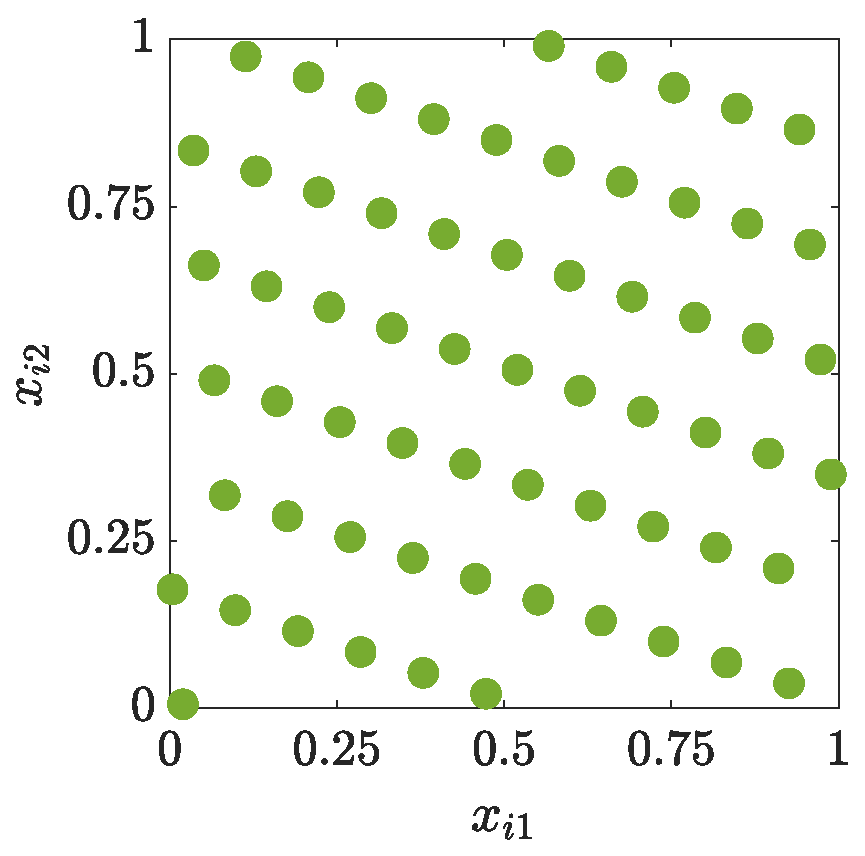
\includegraphics[height = 4.5cm]{ShiftedLatticePoints.eps} \qquad	
    \includegraphics[height = 4.5cm]{"optPrice_guaranteed_time_full_Baker_d12_r1_2018-Sep-6"}
    \caption{An example of shifted integration lattice nodes in two dimensions (left). The performance of of Bayesian cubature for an option pricing example (right).}
    \label{fig:latfig}
\end{figure}

Under these assumptions one may express \eqref{JHFullBayes} and \eqref{thetaEB} in terms of the fast transforms of the integrand data and the first column of the matrix $\vC_0$ (\JH, Sections 3.2, 3.3):
\begin{subequations} \label{JHFullBayesFast}
\begin{align}
\label{FastTrans}
\tvf & : = \vV^{H} \vf, \qquad \vlambda = \diag(\vLambda) = \tilde{\vC}_1 := \vV^{H} \vC_1, \\
    \hat{\Pi}[f] & =  \Ex_n[\hat{\Pi}[g]] = \frac 1n \sum_{i=1}^n f(\vx_i) = \frac{\tf_1}{n} \qquad \text{the sample average},\\
\Var_n[\Pi[g]] & = \frac{1}{n(n-1)} \left(\frac{\lambda_1}{n}  - 1  \right)\sum_{i=2}^n \frac{\bigl \lvert \tf_i\bigr \rvert^2}{\lambda_i} , \\
\label{thetaEBfast}
\vtheta_{\textup{EB}} &= 
\argmin_{\vtheta}
\left[
\log\left(
\sum_{i=2}^n \frac{\abs{\widetilde{y}_i}^2}{\lambda_i}
\right)  
  + 
\frac{1}{n}\sum_{i=1}^n \log(\lambda_i)
\right].
\end{align}
\end{subequations}
Apart from the computations in \eqref{FastTrans}, which require $\Order(n \log n)$ operations, all other calcuations in \eqref{JHFullBayesFast} require only $\Order(n)$ operations.

Section 5 of \JH presents the results of several numerical experiments for Bayesian cubature with shift-invariant kernels and lattice nodes sets.  We reproduce one such experiment in Figure \ref{fig:latfig} (right).  The integrand is the payoff of an arithmetic mean Asian option.  The covariance function is the one given by \eqref{the_kernel_eqn_bernoulli} with $r=1$.  A low degree of smoothness seems is chosen in view of the discontinuities in the partial derivatives of the integrand.  The value of $\gamma$ is determined by empirical Bayes as in \eqref{thetaEBfast}.  The sample size, $n$, is increased in a sequence of powers of $2$ until the stopping criterion implied by \eqref{BCFullStop}, whose terms are computed quickly via \eqref{JHFullBayesFast}, is satisfied.  Four different values of the tolerance were tried, $\varepsilon = 0.1, 0.01, 0.001,$ and $0.0001$. The aim is for the cubature error, $|\Pi[f] - \hat{\Pi}[f]|$, to me no greater than, but not too much less than, the prescribed tolerance nearly all the time.  In this experiment, the error tolerance is always met.  As expected, the computation time is less for larger tolerances and greater for smaller tolerances.  

In this example, and others provided in Section 5 of \JH, the cost of evaluating the integrand is modest, and so the cost of obtaining the needed function data, $\vf$ is on the same order as the matrix-vector operations required to compute the credible interval.  \JH also provides examples of the empirical Bayes and generalized cross-validation approaches to determining the parameters inherent in the covariance function and to using credible intervals as stopping criteria for Bayesian cubature.  All of these approaches are successful, which suggests that they should be explored over a larger range of examples.  

\section{Probabilistic Versus Deterministic} \label{sec:ProbDet}

Section 3.2 in \BOGOS sets the covariance kernel, $c$, for the Gaussian process, $g$, identical to the reproducing kernel, $k$, of the Hilbert space containing the integrand, $f$ for ``aesthetic'' reasons.  While this makes the application of several results from numerical analysis of deterministic cubature more readily transferable to Bayesian cubature, we think that such a correspondence muddies the waters.  While there are mathematical similarities between the probabilistic and determinstic approaches to cubature, there are some important differences.  

When the optimal cubature weights are used, the deterministic error bound in \eqref{HJErrBd} may be expressed as
\begin{subequations} \label{HJErrBdTight}
\begin{gather} 
    \label{HJErrBdBdTight}
    \bigl \lvert \hat{\Pi}[f] - \Pi[f] \rvert^2 \le \lVert f - S(f) \rVert_{\calH}^2 \ \bigl \{ \Pi\Pi[k(\cdot,\cdot)] - \Pi[\vk(\cdot, X)]\vK^{-1} \Pi[\vk(X,\cdot)]\bigr \} , \\
    \label{HJErrbdTightCub}
    \text{where } \hat{\Pi}[f] = \Pi[S(f)] = \Pi[\vk(\cdot, X)] \vK^{-1} \vf,
\end{gather}
\end{subequations}
and $S(f)$ is the minimum Hilbert space norm interpolant of the integrand, $f$.  The reason that $\lVert f \rVert_{\calH}$ in \eqref{HJErrBd} can be replaced by $\lVert f - S(f) \rVert_{\calH}$ is that the cubature in \eqref{HJErrbdTightCub} integrates $S(f)$ exactly. Moreover, $f - S(f)$ is orthogonal to $S(f)$ with respect to the the Hilbert space inner product.  Also note that
\begin{equation} \label{HJErrBdTight}
   \lVert S(f) \rVert^2_{\calH} = \vf^T \vK^{-1} \vf.
\end{equation}

Compare this to Proposition 2 of \BOGOS, which states that 
\begin{subequations} \label{HJBCErrBdTight}
\begin{gather} 
\label{HJBCErrbdTightCub}
    \hat{\Pi}[f] = \Ex[\Pi[g]] = \Pi[\vc_0(\cdot, X)] \vC_0^{-1} \vf , \\
    \label{HJBCErrBdBdTight}
    \Var[\Pi[g]] = \frac{\vf^T \vC_0^{-1} \vf}{n} \ \bigl \{ \Pi\Pi[c_0(\cdot,\cdot)] - \Pi[\vc_0(\cdot, X)]\vC_0^{-1} \Pi[\vc_0(X,\cdot)] \bigr \} , \\
    \text{where } \hat{\Pi}[f] = \Pi[S(f)] = \Pi[\vk(\cdot, X)] \vK^{-1} \vf,
\end{gather}
\end{subequations}
The formulas for the cubature $\hat{\Pi}[f]$ in both the deterministic and probabilistic senses are identical if $k$ is identical to $c_0$.  They are also independent of the vertical scale factor multiplying inherent in the definition of $k$ or $c_0$, i.e., the reproducing kernel $k$ and $47k$ yield the same cubature rule.  Likewise, the bound on the squared error in \eqref{HJErrBdBdTight} and the variance of the integral of the stochastic process in \eqref{HJBCErrBdBdTight} both contain a common factor if $k$ is identical to $c_0$.


Add some more


The sample space for the integrand, $f$, and the Gaussian process used to model the integrand, $g$, need not be directly tied to the 


\section{Hi}


For one-dimensional integration, the standard quadrature algorithms, e.g., in MATLAB \citep{MAT9.5}, expect an input of $\varepsilon$ and adaptively determine the sample size, $n$, required.




\section*{Acknowledgements}
And this is an acknowledgements section with a heading that was produced by the
$\backslash$section* command. Thank you all for helping me writing this
\LaTeX\ sample file.

\bibliographystyle{imsart-nameyear}
\bibliography{FJH23,FJHown23}



\end{document}
